\section{Introduction}


% the license
\begin{frame}{Da Vinci surgical robot}{}

\begin{columns}[T]
\begin{column}{1\textwidth}

  \begin{itemize}
    \item<1-> Minimally invasive surgery
    \vspace{0.3cm}
    \item<2-> Telemanipulation  
    \vspace{0.3cm}
    \item<3-> Only visual feedback  
  \end{itemize}
  
  \begin{figure}[H]
  	\centering
  	\onslide<1->  \begin{subfigure}{0.6\textwidth}
  		\centering
  		\includegraphics[width=1\textwidth]{Billeder/Dan/davinci.jpg}
  	\end{subfigure}
  
  	
  	
  \end{figure}
\end{column}%

\end{columns}


\end{frame}



%%%%%%%%%%%%%%%%%%%%%%%%%%%%%%%%%%%%%%%%%%%%%%%%%%%%%%%%%%%%%%%%%%%%%%%%%%%%%%%%%%%

\begin{frame}{Improvement by haptic feedback}{}


  \begin{itemize}
    \item<1-> Haptic feedback can reduce the number of surgical errors
  \end{itemize}

\begin{figure}
	\includegraphics[width=0.2\textwidth]{Billeder/Dan/console.jpg}
	\hspace{16.3 mm} $\Rightarrow $
	\includegraphics[width=0.2\textwidth]{Billeder/GT.png}
\end{figure}

\resizebox{\textwidth}{!}{
	\begin{tikzpicture}
	
	
	\node[box] (Opt) at (0,0) {Operator};
	\node[box] (Geo) at ($(3,0) + (Opt)$) {\includegraphics[width=0.2\textwidth]{Billeder/GT.png}};
	\node[box] (ros) at ($(3,0) + (Geo)$) {Computer};
	\node[box] (davin) at ($(3,0) + (ros)$) {\includegraphics[width=0.2\textwidth]{Billeder/Dan/sbRIO9636.png}};
	\node[box] (end) at ($(3,0) + (davin)$) {\includegraphics[width=0.2\textwidth]{Billeder/endo2.png}};
	
	
	\draw[->, ultra thick] ([yshift=0.3cm]Opt.east) -- ([yshift=0.3cm]Geo.west);
	\draw[->, ultra thick] ([yshift=0.3cm]Geo.east) -- ([yshift=0.3cm]ros.west);
	\draw[->, ultra thick] ([yshift=0.3cm]ros.east) -- ([yshift=0.3cm]davin.west);
	\draw[->, ultra thick] ([yshift=0.3cm]davin.east) -- ([yshift=0.3cm]end.west);
	
	
	\draw[<-, ultra thick] ([yshift=-0.3cm]Opt.east) -- ([yshift=-0.3cm]Geo.west);
	\draw[<-, ultra thick] ([yshift=-0.3cm]Geo.east) -- ([yshift=-0.3cm]ros.west);
	\draw[<-, ultra thick] ([yshift=-0.3cm]ros.east) -- ([yshift=-0.3cm]davin.west);
	%\draw[<-, ultra thick] ([yshift=-0.3cm]davin.east) -- ([yshift=-0.3cm]end.west);
	
	\node at (1.5,1.3) {Position};
	\node at (4.5,1.3) {Position};
	% \node at (7.5,1) {yes};
	% \node at (10.5,1) {yes};
	
	\node at (1.5,-1.3) {Force};
	\node at (4.5,-1.3) {Force};
	\node at (10.5,1.3) {Torque};
	% \node at (10.5,1) {yes};
	%\node at (7.5,1.5) {Motor enable};
	\node at (7.5,1.3) {Position};
	\node at (7.5,-1.3) {Position};
	\node at (7.5,-1.8) {Velocity};
	\node at (7.5,-2.3) {Current};
	
	\end{tikzpicture}
}

 \end{frame}




%%%%%%%%%%%%%%%%%%%%%%%%%%%%%%%%%%%%%%%%%%%%%%%%%%%%%%%%%%%%%%%%%%%%%%%%
\section{Control Scheme}




\begin{frame}{Control Architecture}{}
  \begin{itemize}
    \item<1-> Two closed loops send reference signals mutually
    \item<2-> The architecture contains delays
    \item<3-> The force is estimated from the measured current
    \end{itemize}
    
    \includegraphics[width=\textwidth]{Billeder/Dan/control.pdf}
\end{frame}

